% This template is based off one created by:
% Pascal Bercher, pascal.bercher@anu.edu.au (Version 1.00, 2021/12/03)

%----------------------------------------------------
% Document Set-up
%----------------------------------------------------
\documentclass[a4paper,twoside,cleardoublepage=plain,bibliography=totoc,headings=openany]{scrarticle}

% Margins and Title Page
\usepackage[a4paper, margin=2.5cm]{geometry}

% Standard Mathematics Packages
\usepackage{amssymb,amsthm,amsmath,bbold,graphicx}

% Referencing and formatting links
\usepackage{xurl}
\usepackage[backref=page]{hyperref}
\hypersetup{
  linktocpage, % in the table of contents, the numbers serve as links, not the entries
  colorlinks  = true, % the items are colored instead of colored boxes around them
  urlcolor    = cyan,
  linkcolor   = red,
  citecolor   = blue
}
% the following makes back references more appealing.
% Taken from: https://tex.stackexchange.com/questions/183702/formatting-back-references-in-bibliography-bibtex
\renewcommand*{\backref}[1]{}
\renewcommand*{\backrefalt}[4]{[%
\ifcase #1 Not cited.%
  \or Cited on page~#2.%
  \else Cited on pages #2.%
\fi]}
\usepackage{cleveref}

% Date and Time
\usepackage{datetime}
\newdateformat{monthonly}{\monthname[\THEMONTH]}

% Placement
% \usepackage{float}
\usepackage{floatrow} % allows to place a caption next to a figure
\floatsetup[table]{capposition=top} %  forces table captions to appear on top.
\usepackage{caption}
\usepackage{subcaption}

% Tables and Matrices
\usepackage{booktabs} % for tables that actually look nice!
\usepackage{multirow}
\usepackage{array}

% Boxing
\usepackage{mdframed}

% Indentation
\usepackage{parskip} % when this is included, no indentations are used for new paragraphs, and instead paragraphs are separated by a small distance between them

% Lists
% \usepackage{enumitem}
% \setlist[enumerate,1]{label={(\roman*)}}
\usepackage{paralist} % provides compactitem, a more compact itemize

% Fancy Figures
\usepackage{tikz}
\usetikzlibrary{matrix}
\usetikzlibrary{arrows}

% Algorithms
\usepackage[ruled,vlined]{algorithm2e}

% Bibliography
\usepackage[semicolon, square, numbers]{natbib} % a specific citation style
\bibliographystyle{plainnat}

% % Formatting Chapter Title Pages
% \usepackage{titlesec} % used to add those horizontal lines around chapter package; see defs below.
% \usepackage[standardsections]{scrhack} % fixes an error causes by loading titlesec for class scrbook
% % [requires titlesec]
% % Surrounds all chapter titles by lines (see screenshot),
% % which includes the titles in the TOC and list of figures and tables
% \titleformat{\chapter}[display]
% {\bfseries\huge}
% {\filleft\Large\chaptertitlename~\thechapter}
% {3ex}
% {\titlerule\vspace{1.5ex}\filright}
% [\vspace{1ex}\titlerule]

% \renewcommand{\chaptername}{Chapter}

% fixes a compilation error that otherwise occurs in combination with scrbook
% see https://tex.stackexchange.com/questions/625083/adding-horizontal-line-before-and-after-chapter-heading-in-scrbook
% \titleformat{\section}
%  {\normalfont\Large\bfseries}{\thesection}{1em}{}
% \titleformat{\subsection}
%  {\normalfont\large\bfseries}{\thesubsection}{1em}{}
% \titleformat{\subsubsection}
%  {\normalfont\normalsize\bfseries}{\thesubsubsection}{1em}{}
 
%----------------------------------------------------
% Configurations and Macros
%----------------------------------------------------

% Set your name:
\newcommand{\AuthorName} {Edmund Hofflin and Hannes Gubler}

\newcommand{\CollabName} {No One}

% Set the title of your work:
%  (Choose an informative and interesting title.)
\newcommand{\Title} {Comparison of Incremental Algorithms and Their Application to Logistic Regression}


% Set the name of your school:
\newcommand{\School} {Institute of Mathematics}
% Set the name of your college:
\newcommand{\College} {College of Basic Sciences}
% Set name of university
\newcommand{\University} {École Polytechnique Fédérale de Lausanne}
% Set local of university
\newcommand{\Location} {~Lausanne~\textbar~Vaud~\textbar~Switzerland}
% Set university logo image path
\newcommand{\Logo} {epfl_logo.png}

% Set your project points:
\newcommand{\Credits} {5}


% Set your semester:
\newcommand{\Semester} {Autumn}
% Set your year:
\newcommand{\Year} {2022}


% Set your degree:
\newcommand{\Degree} {Masters of Mathematics}


% Set your course code and name:
\newcommand{\CourseCode} {MATH-412}
\newcommand{\CourseName} {Statistical Machine Learning}


% Set name of first supervisor:
\newcommand{\FirstProf} {Dr.\ Guillaume Obozinski}

% Set whether there's a second supervisor:
%  (change second line accordingly)
\newif\ifTwoProfs % do not delete this part!
\TwoProfsfalse %true     % or \TwoProfsfalse or comment out

% Set name of second supervisor:
\newcommand{\SecondProf} {Dr.\ Doesn't Exist}
 % to specify data used in the title page
%----------------------------------------------------
% Environments for Mathematics
%----------------------------------------------------

\newcommand{\prf}[1]{
  \begin{quote}
    \begin{proof}
      {#1}
    \end{proof}
  \end{quote}
}

\newtheorem{theorem}{Theorem}[section]
\newtheorem{proposition}{Proposition}[section]
\newtheorem{lemma}{Lemma}[section]
\newtheorem{corollary}{Corollary}[section]
\newtheorem{definition}{Definition}[section]
\newtheorem{assumption}{Assumption}[section]

\newcommand{\thm}[2]{
  \begin{mdframed}
    \begin{theorem}[{#1}]\label{thm:\thetheorem}
      {#2}
    \end{theorem}\noindent
  \end{mdframed}
}

\newcommand{\prp}[2]{
  \begin{mdframed}
    \begin{proposition}[{#1}]\label{prop:\theproposition}
      {#2}
    \end{proposition}\noindent
  \end{mdframed}
}

\newcommand{\lmm}[2]{
  \begin{mdframed}
    \begin{lemma}[{#1}]\label{lemma:\thelemma}
      {#2}
    \end{lemma}\noindent
  \end{mdframed}
}

\newcommand{\cor}[2]{
  \begin{mdframed}
    \begin{corollary}[{#1}]\label{cor:\thecorollary}
      {#2}
    \end{corollary}\noindent
  \end{mdframed}
}

\newcommand{\dft}[2]{
  \begin{mdframed}
    \begin{definition}[{#1}]\label{def:\thedefinition}
      {#2}
    \end{definition}\noindent
  \end{mdframed}
}

\newcommand{\asmpt}[2]{
  \begin{mdframed}
    \begin{assumption}[{#1}]\label{asmpt:\theassumption}
      {#2}
    \end{assumption}\noindent
  \end{mdframed}
}

\newcommand{\qa}[2]{
  \begin{quote}
    \textsc{Question}: {#1} \\
    \textsc{Answer}: {#2}
  \end{quote}
}

\newcommand{\question}[1]{
  \textbf{{#1}}
}

\newcommand{\answer}[1]{
  \textsc{Answer}: {#1}
}

\newcommand{\hint}[1]{
  \textit{Hint: {#1}}
}

\newcommand{\eg}[2]{
  \begin{quote}
    \textsc{Example} - \textsc{{#1}}: {#2}
  \end{quote}
}

\newcommand{\note}[1]{
  \textsc{Note}: {#1}
}

%----------------------------------------------------
% Labelling
%----------------------------------------------------

% Equation labelling
\numberwithin{equation}{section}
\newcommand{\labeq}{\label{eq:\theequation}}

% Algorithm labelling: https://tex.stackexchange.com/questions/113403/how-to-use-nameref-with-algorithm2e
\makeatletter
\let\original@algocf@latexcaption\algocf@latexcaption
\long\def\algocf@latexcaption#1[#2]{%
  \@ifundefined{NR@gettitle}{%
    \def\@currentlabelname{#2}%
  }{%
    \NR@gettitle{#2}%
  }%
  \original@algocf@latexcaption{#1}[{#2}]%
}
\makeatother

%----------------------------------------------------
% Letters
%----------------------------------------------------

% Blackboard Bold Letters

\newcommand{\Z}{\ensuremath{\mathbb{Z}}}
\newcommand{\C}{\ensuremath{\mathbb{C}}}
\newcommand{\R}{\ensuremath{\mathbb{R}}}
\newcommand{\F}{\ensuremath{\mathbb{F}}}
\newcommand{\N}{\ensuremath{\mathbb{N}}}
\newcommand{\Q}{\ensuremath{\mathbb{Q}}}
\newcommand{\A}{\ensuremath{\mathbb{A}}}
\renewcommand{\P}{\ensuremath{\mathbb{P}}}
\newcommand{\E}{\ensuremath{\mathbb{E}}}
\newcommand{\V}{\ensuremath{\mathbb{V}}}

%----------------------------------------------------
% Other Commands
%----------------------------------------------------

\newcommand{\shrug}[1][]{%
\begin{tikzpicture}[baseline,x=0.8\ht\strutbox,y=0.8\ht\strutbox,line width=0.125ex,#1]
\def\arm{(-2.5,0.95) to (-2,0.95) (-1.9,1) to (-1.5,0) (-1.35,0) to (-0.8,0)};
\draw \arm;
\draw[xscale=-1] \arm;
\def\headpart{(0.6,0) arc[start angle=-40, end angle=40,x radius=0.6,y radius=0.8]};
\draw \headpart;
\draw[xscale=-1] \headpart;
\def\eye{(-0.075,0.15) .. controls (0.02,0) .. (0.075,-0.15)};
\draw[shift={(-0.3,0.8)}] \eye;
\draw[shift={(0,0.85)}] \eye;
% draw mouth
\draw (-0.1,0.2) to [out=15,in=-100] (0.4,0.95); 
\end{tikzpicture}}

\newcommand{\la}{\ensuremath{\left\langle}}
\newcommand{\ra}{\ensuremath{\right\rangle}}

\newcommand{\PP}{\ensuremath{\mathcal{P}}}
\newcommand{\beegO}{\ensuremath{\mathcal{O}}}
\newcommand{\ep}{\varepsilon}
\let\emptyset\varnothing
\newcommand{\diff}[1]{\ensuremath{\ \text{d}{#1}}}
\renewcommand{\vec}[1]{\ensuremath{\mathbf{#1}}} % define all your macros here

%----------------------------------------------------
% Top Matter
%----------------------------------------------------

\begin{document}

\pagenumbering{roman}
% only the title page is centered; all other pages are aligned according to books
\newgeometry{left=2.5cm,right=2.5cm,top=4cm}
\thispagestyle{empty}

\newdateformat{monthyeardate}{%
  \monthname[\THEMONTH] \THEYEAR}

\onecolumn

\noindent
\begin{minipage}[t]{6cm}%
{\footnotesize%
\raisebox{-\height}{{\bfseries \University}} \\
\Location}
\end{minipage}%
\hfill%
\begin{minipage}[b]{10cm}%
\hfill\raisebox{-\height}{\includegraphics[height=1 cm]{style/\Logo}}
\end{minipage}

\ \\[1.5em]
\phantom{x} \hfill\parbox[t]{50.75 mm}{\flushright \bfseries \School}\\[6 em]
\hfill

\noindent
\parbox{140mm}{\sffamily \bfseries \huge %
\Title%
}\\[.75 em]
{--- \CourseCode~\textbar~\CourseName~\textbar~(\Semester{} \Year)}\\[3 em]

% Degree\\
% \emph{\Degree}\\[3 em]

\noindent
{\footnotesize \textbf By:}\\
\AuthorName\\[2em]

% \noindent
% {\footnotesize \textbf Collaboration:}\\
% {\footnotesize \CollabName}\\[2em]

\noindent
{\footnotesize \bfseries Professors\ifTwoProfs{}s\fi:}\\
{\footnotesize \FirstProf%
\ifTwoProfs\\\SecondProf\fi}\\[2 em]
\vfill
{\footnotesize \monthyeardate\today}

\restoregeometry

% table of contents (nothing to do for you)
% \renewcommand{\contentsname}{Table of Contents}
% \setcounter{tocdepth}{1}
% \tableofcontents
% \clearpage

%----------------------------------------------------
% Content
%----------------------------------------------------

\pagenumbering{arabic}

\section{Introduction}

In many applications, one has to solve optimisation problems whose objective functions do not permit gradient computations \cite{alarie2021two}. As a result, gradient-free optimization methods that only evaluate the function are required to solve these black-box problems. Zeroth Order Stochastic Gradient Descent (ZO-SGD) is a class of optimisation algorithms that use difference methods to approximate the gradient. The performance of ZO-SGD depends on a variety of hyperparameters and the difference method used. We investigate these dependencies, also explored in \cite{liu2020primer} for black-box deep learning, on simple multilayer perceptrons, putting our focus on the effect of dimensionality on performance and computation time.

% Therefore, researchers had to develop gradient-free optimization methods that could optimize those non-differentiable complex objective functions by only using their evaluations. 

% Zeroth order methods are derivative-free optimization methods which do not require gradient computation. Compared to first-order methods, those methods rely on gradient approximations such as Finite Difference, or any other approximation method which only uses function evaluations to determine the optimal solution. Therefore, those methods enable one to optimize non-differentiable functions. However, computing gradient approximations might become computationally expensive due to numerous function evaluations, but are sometimes the only remaining tool when other optimization methods fail to be applied for a given non-differentiable problem.

% In particular, Section \ref{subsec:ZO-SGD} describes Zeroth order Stochastic Gradient Descent (ZO-SGD), which is an extension for non-differentiable functions of the original SGD algorithm. In Section \ref{sec:exp}, we apply the ZO-SGD method to the Iris dataset. Lastly, Section \ref{sec:conclusion} concludes with take-home messages and the next steps regarding this project.

\section{Algorithms}

\paragraph{Stochastic Gradient Descent}
In many applications, objective functions have the form 
\begin{equation}\label{GeneralProb}
    f(x) = \frac{1}{n}\sum_{i=1}^n f_i(x),
\end{equation}
where $f_i$ is the loss function of the $i$-th observation, and $n$ the number of observations. Stochastic Gradient Descent (SGD) is the preferred algorithm for optimising such functions, balancing low computational cost per step, requiring one $\nabla f_i$ to be computed, and a decent convergence rate of $\mathcal{O}\left(\frac{1}{\epsilon}\right)$ \cite{bottou2018optimization} (see Appendix~\ref{app:formal_algorithms} for the pseudo-code of the algorithm). However, SGD does require gradient computation, which is impossible if $f$ or individual $f_i$ are non-differentiable.
%\subsection{Stochastic Gradient Descent}\label{subsec:SGD}

% Gradient Descent (GD) may become very computationally expensive (see Appendix~\ref{app:formal_algorithms} for pseudo-code). Hence, it might become computationally expensive to compute its gradient (sum of $n$ individual gradients), which is required by the Gradient Descent (GD) algorithm (see Appendix~\ref{app:formal_algorithms} for pseudo-code). Therefore, SGD only computes the gradient of one randomly selected $f_i$ in each iteration, reducing the computational cost of each iteration by over a factor of $n$ (see Appendix~\ref{app:formal_algorithms} for the algorithm). As a result, SGD only has $\mathcal{O}\left(\frac{1}{\epsilon}\right)$ convergence \cite{bottou2018optimization}. To compare with the original GD algorithm, GD would be faster for small $n$, but when $n$ is large (as is the case in many modern machine learning settings), SGD converges faster \cite{TODO}. One can easily see that this method requires gradient computation, which might cause problems when the randomly selected $f_i$ is non-differentiable. Hence, we describe hereunder a Zeroth order version of SGD.

% However, the stochasticity of SGD's method introduces variance into the algorithm and this leads to a significant disadvantage. SGD can only converge to an $\mathcal{O}\left(\eta\right)$-radius ball centered around the local minimum $w^*$, where $\eta$ is the constant step-size \cite{bottou2018optimization}. If $\eta$ varies, either using a step-size scheduler or a line-search, then SGD can converge to the local minimum, but then the rate of convergence reduces to $\mathcal{O}\left(\frac{1}{\epsilon^2}\right)$ \cite{reddi2016stochastic} and so many of its benefits are lost.

%\label{subsec:ZO-SGD}
\paragraph{Zeroth Order Stochastic Gradient Descent}
Zeroth Order Stochastic Gradient Descent (ZO-SGD) is a class of optimisation methods that employ difference methods to approximate a stochastic gradient and then emulate SGD (see Appendix~\ref{app:formal_algorithms} for the pseudo-code of algorithms). There are two categories of difference methods, depending on the number of function evaluations needed: one-point and multi-point methods \cite{liu2018zerothorder}

The one-point estimate can be defined as
\begin{equation}
    \hat{\nabla} f(\bold{x}) = \frac{\phi(d)}{\mu}f(\bold{x}+\mu \bold{u})\bold{u},
\end{equation}
where $\bold{u} \sim P$ is a random direction vector which follows a given distribution $P$, $\phi$ denotes a dimension-linked factor related to the choice of $P$, and $\mu>0$ is a perturbation radius. Typically, $P := \mathcal{N}(\bold{0}_d,\bold{I}_{d\times d})$ or a uniform distribution over the unit sphere such that $P := U(\mathcal{S}(0,1))_{d}$. Based on the choice of $P$, we let $\phi(d)=1$ for $P = \mathcal{N}(\bold{0}_d,\bold{I}_{d\times d})$ and $\phi(d)=d$ for $P = U(\mathcal{S}(0,1))_{d}$.

%Furthermore, if one defines $f_\mu(\bold{x}) = \E_u[f(\bold{x}+\mu \bold{u})]$, one can check the unbiasedness of $\hat{\nabla} f(\bold{x})$ with respect to $\nabla f_\mu$, i.e. $\E_u[\hat{\nabla}f(\bold{x})] = \nabla f_\mu(\bold{x})$, thanks to \cite{berahas2021theoretical,Nesterov2017RandomGM}. However, even though it is unbiased with respect to the expectation of the perturbed objective function's gradient, it is not with respect to its true gradient.

%\paragraph{Multi-point estimate}
The two-point estimate extends the single-point estimate by substracting the evaluation of the objective function at $\bold{x}$, as seen below:
\begin{equation}
    \hat{\nabla} f(\bold{x}) := \frac{\phi(d)}{\mu}\left(f(\bold{x}+\mu \bold{u})-f(\bold{x})\right)\bold{u}
    \label{eq:2.3}
\end{equation}

%which also satisfies the unbiaseness by linearity of the expectation, as long as $\bold{u}$ has zero mean.

%One can now check the mean squared error between the approximation and the true value of the gradient, in order to find the error order \cite{berahas2021theoretical,liu2018zerothorder} :
%\begin{equation}\label{eqn:mse_mult}
%    \E[\| \hat{\nabla}f(\bold{x})- \nabla f(\bold{x}) \|^2_2] %= \|\nabla f(\bold{x})\|^2_2 \mathcal{O}(d) + \mathcal{O}\left(\mu^2\left[\frac{d^3 + d}{\phi(d)}\right]\right)
%\end{equation}
%From \ref{eqn:mse_mult}, one notes that as $\mu$ decreases, the second error term decreases, but one has to be careful when reducing $\mu$ as this might cause stability issues. An important point is that the variance is proportional to the dimension (see first term), and this error is irreducible. To tackle this, variance-reduction extensions of SGD has been created, but will not be discussed in this work.

Additionally, one can use the mini-batch technique, drawing $\{\bold{u}_i\}_{i=1,...,b} \sim P$, and then define the following two-point estimate
\begin{equation}
    \hat{\nabla} f(\bold{x}) := \frac{\phi(d)}{\mu}\sum_{i=1}^b\left(f(\bold{x}+\mu \bold{u}_i)-f(\bold{x})\right)\bold{u}_i
\end{equation}
%which lands the approximation error \cite{berahas2021theoretical}
%\begin{equation}\label{eqn:mse_mult_batch}
%    \E[\| \hat{\nabla}f(\bold{x})- \nabla f(\bold{x}) \|^2_2] = \|\nabla f(\bold{x})\|^2_2 \mathcal{O}(\frac{d}{b}) + \mathcal{O}\left(\frac{\mu^2d^3}{\phi(d)b}\right)+ \mathcal{O}\left(\frac{\mu^2d}{\phi(d)}\right).
%\end{equation}
When the number of function evaluations reaches $d$, one can decide to use coordinate-wise gradient estimate instead of randomly drawing $\bold{u}_i$'s. This yields the coordinate-wise two-point estimate
\begin{equation}
    \hat{\nabla} f(\bold{x}) := \frac{1}{\mu}\sum_{i=1}^d\left(f(\bold{x}+\mu \bold{e}_i)-f(\bold{x})\right)\bold{e}_i,
    \label{eq:2.5}
\end{equation}
where $\{\bold{e}_i\}_{i=1,...,d}$ is the canonical basis of $\R^d$. 

%This yields a lower estimation error of $\mathcal{O}(d\mu^2)$ \cite{berahas2021theoretical}.

% Regarding the ZO-SGD, it resembles its first-order   counterpart, except that the gradient is now computed using one of the previously described estimates, as seen in Appendix \ref{app:formal_algorithms}.

\section{Experiments}\label{sec:exp}
We now investigate the performance of ZO-SGD in an empirical setting, determining whether it is a viable class of optimisation algorithms. We conduct this investigation by assessing the impact of the difference method and hyperparameters $\mu$ and $d$ on the ZO-SGD's proficiency to train multilayer perceptrons (MLPs). Our code can be found on \href{https://github.com/EdmundHofflin/Optimisation_ML_Project}{Github}.

\subsection{Dataset Description}
% PENDIGITS DESCRIPTION - NOT RELEVANT ANYMORE:
% For a meaningful study of MLPs' learning, we trained our models on the pendigits dataset. This dataset of 10,992 instances comprises 17 numeric features describing the handwritten digits 0 to 9 \cite{pendigits}. The set therefore contains a total of 10 well-balanced classes: we verified that each of the classes has at least 1000 samples.\\
% We chose this dataset as it is sizable (the iris dataset, for example, was too small and simple, which led to too fast convergence), but also well suited for standard MLPs: adequate hyperparameter choices can reach accuracies of up to 99 $\%$. Most supervised ML datasets available online contain images, but they pose too much of a challenge for standard MLPs, and we preferred to avoid CNNs or Transformers to better understand the effect of dimensionality on convergence rates.

% IRIS DATASET
We performed our experiments on the Iris dataset, which is a small-size set well adapted for simple testing of multiclass classification. The dataset of 150 instances comprises 4 numeric features, is well-balanced and proved sufficiently complex to explore some interesting trends for the simple two-layer MLPs we studied. We also tested the bigger pendigits dataset (10 992 instances), but the computational cost of ZO-SGD made experiments impractical.

\subsection{Methodology}
We elected to train perceptrons with a single hidden layer, whose dimension we varied. We limited the tests to such simple models to ensure a direct relation between the dimensionality of the problem and the performance of ZO-SGD. We tested two standard activation functions, ReLU and sigmoid. However their results and trends were near identical, so we only present the ReLU results for clarity and to demonstrate ZO-SGD optimising non-differentiable functions. We used a learning rate of $0.01$, $100$ epochs, a batch-size of $32$, and the cross-entropy loss. Additionally, all models were initialised with the same seed.

We varied the dimension of the hidden layer over $\left\{3, 4, 8, 16, 32, 64\right\}$, the perturbation radius hyperparameter $\mu$ over $\left\{1, 10^{-1},10^{-2},10^{-3},10^{-4},10^{-5}\right\}$, and the batch number $b$ over $\left\{1, 10, 10^2, 10^3\right\}$. Finally, for all tests, we compared the multi-batch versions of one-point and two-point, and coordinate ZO-SGD against vanilla SGD. We will omit ``multi-batch" for clarity.

% For a comprehensive and scalable study of the effect of dimensionality on the convergence of our algorithm, we chose to train perceptrons with one hidden layer whose size we varied. \\
% We tested two activation functions for the hidden layer (both for SGD and ZO-SGD learning): ReLU and sigmoid, two standard functions used in the ML community. In both cases we opted for the cross entropy loss: it is a widely used loss for supervised ML problems, and it is non-convex, making the study of its learning dynamics particularly interesting.\\
% We trained our ReLU and sigmoid neural networks with both SGD and ZO-SGD, a learning rate of 0.01, 1000 epochs and a batch size of 64: a few preliminary tests showed that those learning parameters yielded good performance on average. We chose to keep them constant to give more validity to direct comparisons of learning methods and hyperparameters. As explained earlier, we compute SGD on small batches for variance-reduction purposes. \\
% The hyperparameters we did vary during training were: the number of hidden neurons (for the study of the effect of dimensionality on convergence), and the learning radius $\mu$ and N (WHAT IS THIS, DOES NOT APPEAR EARLIER DOES IT???) of the ZO-SGD algorithm.

\subsection{Results}

\paragraph{Batch requirement of one- and two-point methods}
The most immediate result was the high batch $b$ requirement of both the one- and two-point estimation methods. The one-point method was never stable and did not consistently converge, even with $b = 1000$. The two-point method was somewhat stable, converging in roughly $50\%$ of tests with $b = 1000$, but very infrequently with $b = 100$ and never with $b = 1$ or $10$. These results align with the theory: one-point estimate suffers from extremely high variance, slowing or preventing convergence, hence multi-point estimates are almost exclusively used in practice \cite{flaxman2004online}. Given this, we focus our attention hereafter on the two-point estimation method with $b = 1000$ and the coordinate estimation method.

\paragraph{General comparison of two-point and coordinate ZO-SGD and SGD}
Figure~\ref{fig:plot_1} compares these methods against SGD for $\mu = 0.01$ and $d = 4$. We observe that the SGD  has a lower loss than its two other zeroth-order methods. The two-point and coordinate ZO-SGD have similar behaviours, and do not have a high loss reduction over the 100 epochs. Furthermore, the computational time in seconds per epoch was approximately $1$, $0.1$ and $0.001$, for two-point, coordinate, and SGD, respectively. So not only did ZO-SGD converge more slowly than SGD, it required orders of magnitude more computation. While two-point and coordinate estimation variants of ZO-SGD are valid optimization methods, they are significantly slower than SGD, and should therefore be used when only necessary (i.e. when SGD is not available).

\paragraph{Impact of Dimensionality}
% Computational cost linear in d. Much higher than SGD
% Instability of two-point at higher dimensions
% Discuss wrt # hidden layers (and link to high dimensionality)

Figure~\ref{fig:plot_2} shows the results of our study of the effect of dimensionality (varied by changing the number of hidden neurons of our 2-layer network) on convergence and computation time. The left plot of  Figure~\ref{fig:plot_2} shows that SGD and coordinate descent are quite robust methods: they remained stable for the range of dimensions tested. However, the loss of two-point estimates depends heavily on the number of hidden layers, suggesting a stability issue. This instability is not surprising when we know from \cite{liu2020primer} that the variance of mini-batch stochastic gradients for this method is
\begin{equation}\label{eqn:mse_mult_batch}
   \E[\| \hat{\nabla}f(\bold{x})- \nabla f(\bold{x}) \|^2_2] = \|\nabla f(\bold{x})\|^2_2 \mathcal{O}(\frac{d}{b}) + \mathcal{O}\left(\frac{\mu^2d^3}{\phi(d)b}\right)+ \mathcal{O}\left(\frac{\mu^2d}{\phi(d)}\right).
\end{equation}
We can see in this equation that the variance scales with $d^3$, which could explain the instability with increasing dimensions. Coordinate ZO-SGD does not suffer from that problem: the same variance scales with $\mathcal{O}\left(d\mu^2\right)$ for this method.

Figure \ref{fig:plot_2} also shows that both the computation time of the two-point estimate and coordinate descent scale linearly with the dimensionality. This is consistent with theory: we can see from equations \eqref{eq:2.3} and \eqref{eq:2.5} that the complexities of the gradient approximations are respectively of $\mathcal{O}\left(b d\right)$, as we sample $u_i$ from $\R^d$ and $\mathcal{O}\left(d\right)$. SGD theoretically also has a complexity of $\mathcal{O}\left(d\right)$, but that was hardly visible in the experimental plot given its small slope.

\paragraph{Impact of $\mu$}
Figure~\ref{fig:plot_3} shows the relationship between the perturbation radius $\mu$ and the performance of two-point and coordinate estimation methods for ZO-SGD, varying $\mu$ over $\left\{10^{-1}, 10^{-3}, 10^{-5}\right\}$. As evidenced by Equation~\eqref{eqn:mse_mult_batch}, the variance of these difference methods scales with $\mu^2$. However, in Figure~\ref{fig:plot_3}, the coordinate method is seemingly invariant under the changes in $\mu$, and the two-point method only alters its loss trajectory with minimal, if any, change in variance. We suspect that this minimal impact is due to the relative scale of $\mu$: it is several orders of magnitude smaller than $d$, the most significant variance factor, and is potentially even small enough to be comparable to numerical errors. Therefore, at this scale we conclude that $\mu$ is a less significant hyperparameter than $d$ for the performance of ZO-SGD methods.

\section{Conclusion}\label{sec:conclusion}
In this project, we assessed and compared various zeroth-order methods for SGD. While those methods are valid optimization methods, they are extremely slow, and do not cope with dimensionality increases. Their usage should therefore be kept only for problems where the already existing first-order methods do not work, as a last resort. From our literature review, we noted that no empirical comparison of computation time with respect to the dimensionality was done. Hence, Figure \ref{fig:plot_2} and its analysis is our main contribution to the subject.

Next steps of this work would be to assess the impact of the number of samples on computation time and loss for the ZO-SGD methods, and try to use those methods for other types of ML algorithms.

%----------------------------------------------------
% End Matter
%----------------------------------------------------

% Literature
\bibliography{mybib.bib}

% Appendix
\appendix
\section{Formal Algorithms}\label{app:formal_algorithms}
In this section, we present the algorithms GD and SGD to solve \eqref{GeneralProb}.

\begin{algorithm}[H] 
    \caption{Gradient descent}
    \KwIn{$\mathbf{w}_0 \in \mathbb{R}^p$ as starting point, stepsize $\eta$.}
    \For{k = 0,1,2,...}{
        Set $\mathbf{w}_{k+1} = \mathbf{w}_k - \eta \nabla P(\mathbf{w}_k)$ \\
    }
\end{algorithm}

\begin{algorithm}[H]
    \caption{Stochastic gradient descent}
    \KwIn{$\mathbf{w}_0 \in \mathbb{R}^p$ as starting point, stepsize $\eta$.}
    \For{k = 0,1,2,...}{
        Select $i \in \{1,...,n\}$ uniformly at random. \\
        Set $\mathbf{w}_{k+1} = \mathbf{w}_k - \eta \nabla f_i(\mathbf{w}_k)$ \\
    }
\end{algorithm}

\begin{algorithm}[H]
    \caption{Zeroth order stochastic gradient descent}
    \KwIn{$\mathbf{x}_0 \in \mathbb{R}^p$ as starting point, stepsize $\eta$, and the gradient estimation function $\psi(\cdot,\phi,\mu)$.}
    \For{k = 0,1,2,...}{
        Select $i \in \{1,...,n\}$ uniformly at random. \\
        Set $\hat{\nabla}f_i(\mathbf{x}_k) := \psi(f_i,\mathbf{x}_k,\phi,\mu)$\\
        Set $\mathbf{x}_{k+1} = \mathbf{x}_k - \eta \hat{\nabla}f_i(\mathbf{x}_k)$ \\
    }
\end{algorithm}

\section{Plots of Results}\label{app:plots}
In this section, we present plots that evidence our results in Section~\ref{sec:exp}

\begin{figure}[H]
    \centering
    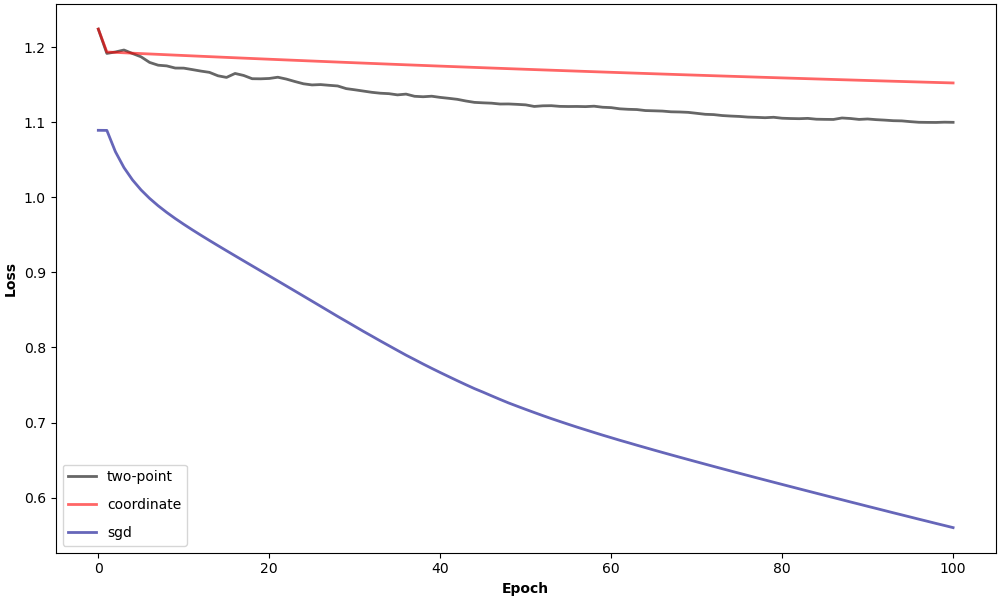
\includegraphics[width=\linewidth]{assets/plot_1.png}
    \label{fig:plot_1}
    \caption{Comparison of loss over epochs of Two-Point and Coordinate Estimation variants of ZO-SGD and SGD with Hidden Dimension $d = 4$ and $\mu = 0.01$. SGD performs better regarding the two other methods over epochs.}
    \label{fig:plot_1}
\end{figure}

\begin{figure}[H]
    \centering
    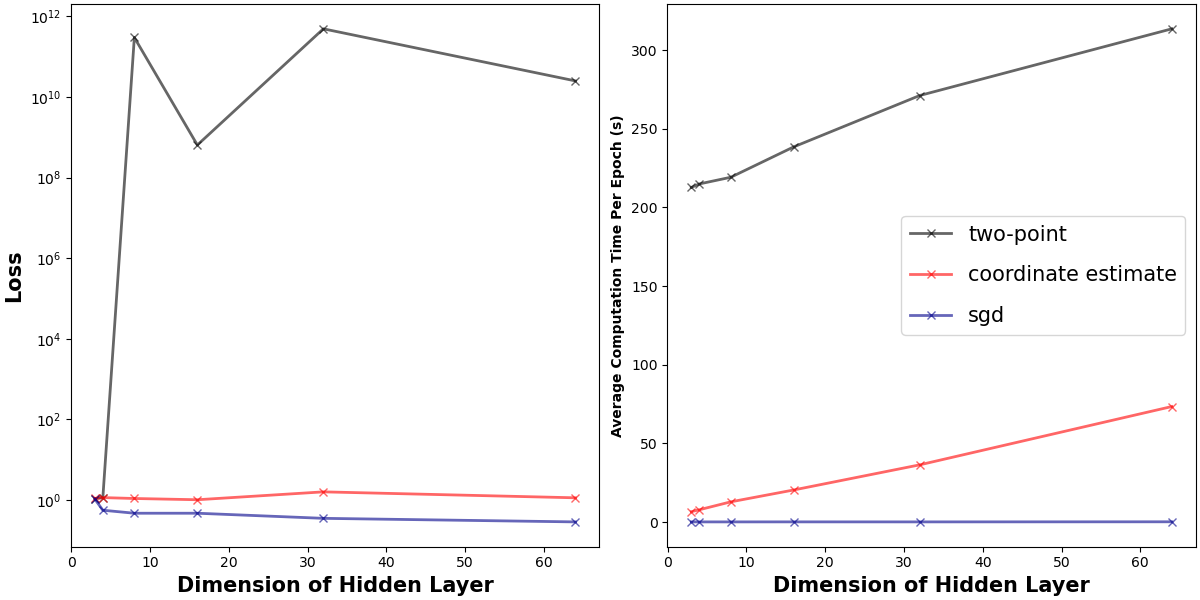
\includegraphics[width=\linewidth]{assets/plot_2.png}
    \caption{Impact of hidden layer dimension on the loss and computational time of two-point and coordinate estimation variants of ZO-SGD and SGD with $\mu = 0.01$. The left plot suggests that two-point estimates are quickly destabilised by high dimensionality, whereas coordinate descent and SGD look robust. The right plot on the other hand shows that the three algorithms scale linearly with dimensionality, but with very different coefficients: dimensionality is more problematic for two-point and coordinate estimates.}
    \label{fig:plot_2}
\end{figure}

\begin{figure}[H]
    \centering
    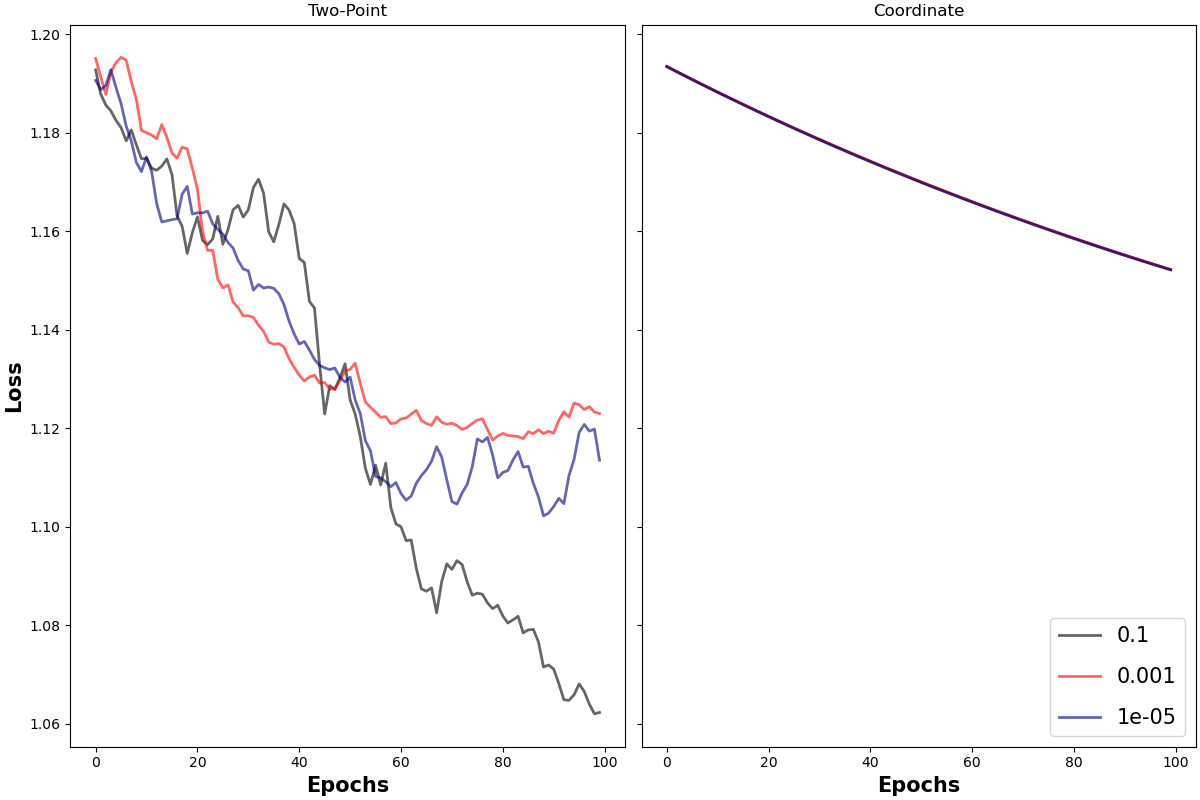
\includegraphics[width=\linewidth]{assets/plot_3.png}
    \caption{Relationship between the perturbation radius $\mu$ and the performance of two-point and coordinate estimation methods for ZO-SGD, varying $\mu$ over $\left\{10^{-1}, 10^{-3}, 10^{-5}\right\}$. The left plot show the loss trajectory of the two-point method, showing small but relatively insignificant changes. The right plot shows the loss trajectory of the coordinate method, showing no noticeable changes. Overall, at these scales, the impact of $\mu$ is minimal.}
    \label{fig:plot_3}
\end{figure}

\end{document}
